\documentclass[10pt,a4paper]{article}
\usepackage[utf8]{inputenc}
\usepackage{amsmath}
\usepackage{amsfonts}
\usepackage{amssymb}
\usepackage{listings}
\usepackage{intex}
\usepackage{hologo}
\usepackage{enumitem}
\usepackage{fancyvrb}

\VerbatimFootnotes

\newcommand{\bs}{\textbackslash}%
\newcommand{\ls}{\textless}%
\newcommand{\gr}{\textgreater}%

\author{G. A. Oliveira}
\title{The \intexs toolkit}

\begin{document}
\maketitle
\section{Introduction}
This is the user-manual for \intex, a typesetting system for interactive-document writing.
\section{Overview}
Figure \ref{fig:flow} shows the steps to generate an interactive document using \intex. They are:
\begin{enumerate}[label*=\arabic*.]
	\item First of all we work in our \TeX\space document and compile it to obtain a PDF file.
	\begin{enumerate}[label*=\arabic*.]
		\item Import \verb|intex.sty| package to create a new class environment and use its definitions to insert special content into the document .
		\item Compile the \verb|.tex| main file using \Hologo{pdfLaTeX} with option \verb|--enable-18|. This option is necessary to convert an expression in math mode to a static image in order to preserve its shape.\footnote{If you are using a \TeX\space editor, it may be possible to configure it to use this option automatically.}
		\item As result, we obtain a PDF file with a placeholder for each content insertion. The metadata is carried as hyperlink reference.
	\end{enumerate}
	\item In this part we process the PDF file obtained in last step to obtain a HTML document in which each placeholder is replaced by its actual content.
	\begin{enumerate}[label*=\arabic*.]
		\item The PDF file is optimized using \verb|Ghostscript| and converted to HTML using \verb|pdf2htmlEX|.
		\item As result, we obtain an HTML and some auxiliary files. There's an \verb|img| element for each placeholder and its metadata is carried in the \verb|href| property.
		\item The HTML is processed by a Python application in which every content entry has its placeholder element replaced according to its class.\footnote{Currently, only the classes 'iframe' and 'video' are supported. They store its \verb|src| property as metadata and are replaced by an \verb|iframe| element. Soon it will be possible for users to define their own replacement directives.}
		\item Finally we obtain our interactive document ready to be distributed over the web.
	\end{enumerate}
\end{enumerate}

\begin{figure}
\centering
	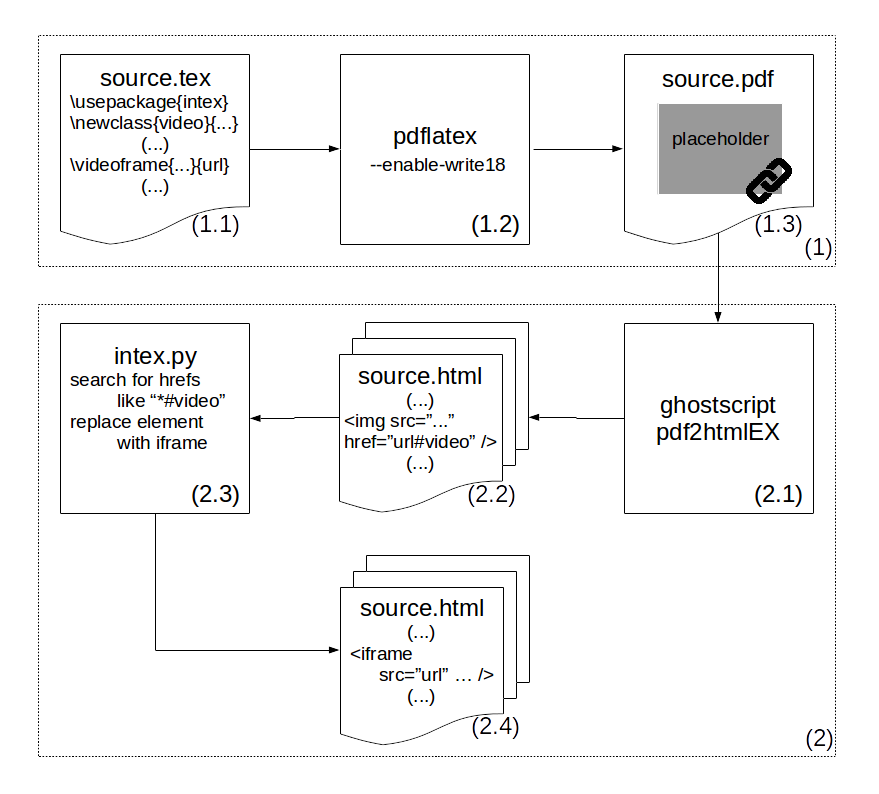
\includegraphics[width=.7\textwidth]{flow.png}
\caption{Workflow to generate an interactive document using \intex}
\label{fig:flow}
\end{figure}

\section{A working example}
\subsection{Setting up}
Let's initiate a new class called \verb|applet|.
\begin{lstlisting}[frame=single]
\newclass{applet}{Applet}{List of applets}
\end{lstlisting}
\newclass{applet}{Applet}{List of applets}
Now we are able to include applet frames along the document. There are two approaches for doing this.
\subsection{Inserting content}
\subsubsection{The easy way}
If you are not a \TeX skilled user nor familiar to \intex, it's probably the best way for you to get started. There are a few short commands to insert content frames with default layout that should fit in most use cases.
\clearpage
To insert a content frame with an empty placeholder we call: 
\begin{lstlisting}[frame=single]
\appletframe{.8}{.5}{https://...}
\end{lstlisting}
\appletframe{.8}{.5}{https://www.geogebra.org/material/iframe/id/HjsJy8FV}
To insert the same frame with caption, use:
\begin{lstlisting}[frame=single]
\appletframe{.8}{.5}{https://...}{Theorem of Thales}
\end{lstlisting}
\appletframecap{.8}{.5}{https://www.geogebra.org/material/iframe/id/HjsJy8FV}{Theorem of Thales}
\clearpage
Now let's say you want your document to be meaningful in its static version. It can be done by inserting images instead of empty placeholders. Although the images will remain static in the PDF version, they can point to the url source link. This kind of frames can be inserted with:
\begin{lstlisting}[frame=single]
\appletgframe[width=.8\textwidth]{ggb.png}{https://...}
\end{lstlisting}
\appletgframe[width=.8\textwidth]{ggb}{https://www.geogebra.org/material/iframe/id/fzdctpmJ}
Likewise, to get a frame with caption we call:
\begin{lstlisting}[frame=single]
\appletgframecap[width=.8\textwidth]{ggb.png}{https://...}
\end{lstlisting}
\appletgframecap[width=.8\textwidth]{ggb}{https://www.geogebra.org/material/iframe/id/fzdctpmJ}{Circumcircle of a triangle}
\subsubsection{The (not so) hard way}
If the content frame is not placed where you want it to be or you are not satisfied with its layout and appearence, you should do take this way instead. Basically, it works like including a graphic using \verb|graphicx| inside a \verb|figure| environment. Consider the following code that shows how it works for the \verb|applet| class we've 
\begin{lstlisting}[frame=single]
\begin{applet}[H]
  \centering
  \includeapplet{.8\textwidth}{.5\textwidth}{https://...}
\end{applet}

\begin{applet}[H]
  \centering
  \includegapplet[width=.8\textwidth]{ggb.png}{https://...}
  \caption{Circumcircle of a triangle again}
\end{applet}
\end{lstlisting}
\begin{applet}[H]
\centering
\includeapplet{.8\textwidth}{.5\textwidth}{https://www.geogebra.org/material/iframe/id/HjsJy8FV}
\end{applet}
\begin{applet}[H]
\centering
\includegapplet[width=.8\textwidth]{ggb.png}{https://www.geogebra.org/material/iframe/id/fzdctpmJ}
\caption{Circumcircle of a triangle again}
\end{applet}
Since \verb|applet| is a \verb|float| environment, it accepts the same options and behaves as any other environment of this type. The command \verb|\includegapplet| accepts the same options as \verb|\includegraphics| from \verb|graphicx| package.
\subsection{Making the list-of}
You can easily make the table of contents for the \verb|applet| environment by calling:
\begin{lstlisting}[frame=single]
\listofapplet
\end{lstlisting}
\listof{applet}{List of applets}

\end{document}
